\documentclass[a4paper]{article}
\usepackage[utf8]{inputenc}
\usepackage{hyperref}

% the following were all needed for the table (!)
\usepackage{amssymb} % for \checkmark
\usepackage{array}
\usepackage{color}
\usepackage{makecell}
\usepackage{colortbl}
% end of packages needed by the table

% For the figures based on images:
\usepackage{graphicx}
\graphicspath{{img/}}
% end

% For the code listings
\usepackage{listings}
\definecolor{codegreen}{rgb}{0,0.6,0}
\definecolor{codegray}{rgb}{0.5,0.5,0.5}
\definecolor{codeblack}{rgb}{0,0,0}
\definecolor{codepurple}{rgb}{0.58,0,0.82}
\definecolor{codeblue}{rgb}{0,0,0.6}
\definecolor{backcolour}{rgb}{0.95,0.95,0.95}
 
\lstdefinestyle{python}{
    backgroundcolor=\color{backcolour},   
    commentstyle=\color{codegreen},
    keywordstyle=\color{codeblue},
    numberstyle=\tiny\color{codegray},
    stringstyle=\color{codepurple},
    basicstyle=\footnotesize\ttfamily,
    breakatwhitespace=false,         
    breaklines=true,                 
    captionpos=t,
    keepspaces=true,                 
    language=Python,
    numbers=left,                    
    numbersep=5pt,                  
    showspaces=false,                
    showstringspaces=false,
    showtabs=false,                  
    tabsize=2
}

\lstdefinestyle{json}{
    backgroundcolor=\color{backcolour},   
    commentstyle=\color{codeblack},
    keywordstyle=\color{codeblack},
    numberstyle=\tiny\color{codeblack},
    stringstyle=\color{codeblack},
    basicstyle=\footnotesize\ttfamily,
    breakatwhitespace=false,         
    breaklines=true,                 
    captionpos=b,
    keepspaces=true,                 
    language=Python,
    numbers=none,                    
    showspaces=false,                
    showstringspaces=false,
    showtabs=false,                  
    tabsize=2
}
% end


\title{A BigchainDB Primer}
\author{BigchainDB GmbH, Berlin, Germany}
\date{May 2017}

\begin{document}

\maketitle

\begin{abstract}
BigchainDB is a scalable blockchain database:
a big-data database with blockchain characteristics
including decentralization, immutability and
built-in support for creation \&~transfer of assets.
Decentralized protocols and technologies have always been a part of the Internet,
but the introduction of Bitcoin ignited a new wave of interest in their capabilities.
In particular, Bitcoin showed that it's possible to create a trustable, immutable
record of transactions (a ledger) without relying on a central, trusted third party.
Many people realized that the ideas (``blockchain technologies'') behind Bitcoin
could be used, in theory, to store trustable records of any kind.
Unfortunately, Bitcoin itself can't scale to handle all those records,
at least not in its current form.
There are many ideas and prototypes to scale Bitcoin and similar blockchains.
BigchainDB takes a different approach to solving the scaling problem.
It starts with a proven, scalable, big-data database,
then adds blockchain characteristics.
\end{abstract}


\section{Overview}

BigchainDB is a scalable blockchain database:
a big-data database with blockchain characteristics
including decentralization, immutability and
built-in support for creation \&~transfer of assets.
This primer explains why something like BigchainDB was needed,
summarizes how it adds blockchain characteristics,
explores how it fits into the rest of the decentralization ecosystem,
and concludes with a section about how you can try it.


\section{Bitcoin and Other Decentralized Protocols}

One goal of the early Internet (ARPAnet) was to create a communications network
that could withstand nuclear war~\cite{arpanet_and_nuclear_war}.
To meet that goal, the designers removed the need for a central owner or
controller, a single point of failure. The Internet is decentralized.
Many other Internet-based protocols are similarly decentralized,
at least in part, e.g.~email, DNS, and BitTorrent.
Bitcoin~\cite{nakamoto2009bitcoin}, introduced in 2009,
is also a decentralized protocol,
but it sparked a new wave of interest in such protocols.
The reason was that it demonstrated a working decentralized cryptocurrency
requiring no central bank or other trusted third party.
Trust emerges from the protocol and its one lasting artifact:
the long-term Bitcoin blockchain---a record
of every valid/finalized bitcoin transaction,
copied consistently and verifiably to thousands
of computers all over the world.


\section{Blockchains for Records of Other Things?}

If Bitcoin can generate a trustable record of bitcoin transactions,
without needing a central owner or controller,
could Bitcoin or similar be used
to generate a trustable record of other trust-important information?
Consider
birth certificates,
college transcripts,
patent filings,
land ownership transactions,
art ownership transactions\footnote{BigchainDB
began as a project within within ascribe.io,
which offers a service to record art attribution, transfer,
consignment and loan records on the Bitcoin blockchain.},
supply-chain records,
lab reports,
or
government transparency reports.
Some of those examples
generate a lot of records very fast.
How much could Bitcoin handle?


\section{The Scale of Bitcoin vs. Modern Databases}

The Bitcoin network of today records less than ten transactions per second (on average),
and adding more nodes won't change that: write throughput doesn't scale with node count.
One \emph{can} store arbitrary information in a Bitcoin transaction,
but not much: dozens of bytes.
The total storage capacity of the Bitcoin blockchain grows
by about 1~MB every 10~minutes, but that's \emph{all} the data, not just the arbitrary data.
Moreover, total storage capacity \emph{doesn't} grow when more nodes are added to the network.
It takes tens of minutes to hours before a Bitcoin transaction can be considered finalized
(i.e.~part of the long-term blockchain).

Now consider a typical modern ``big-data'' database.
Write throughput can be in the millions of transactions per second (or more),
and it can grow when you add more nodes.
For example, Netflix tested Cassandra in 2011 and the results
are shown in Figure~\ref{fig:cassandra_throughput}.
At the bottom left of the plot, we see that $50$ distributed Cassandra nodes could handle $174,000$ writes per second.
Increasing to $300$ nodes allowed for $1.1$ million writes per second~\cite{cockcroft2011benchmarking}.
A follow-up study three years later showed a throughput of $1$ million writes per second with just a few dozen nodes~\cite{kalantzis_netflix}.


\begin{figure}[!ht]
  \centering
  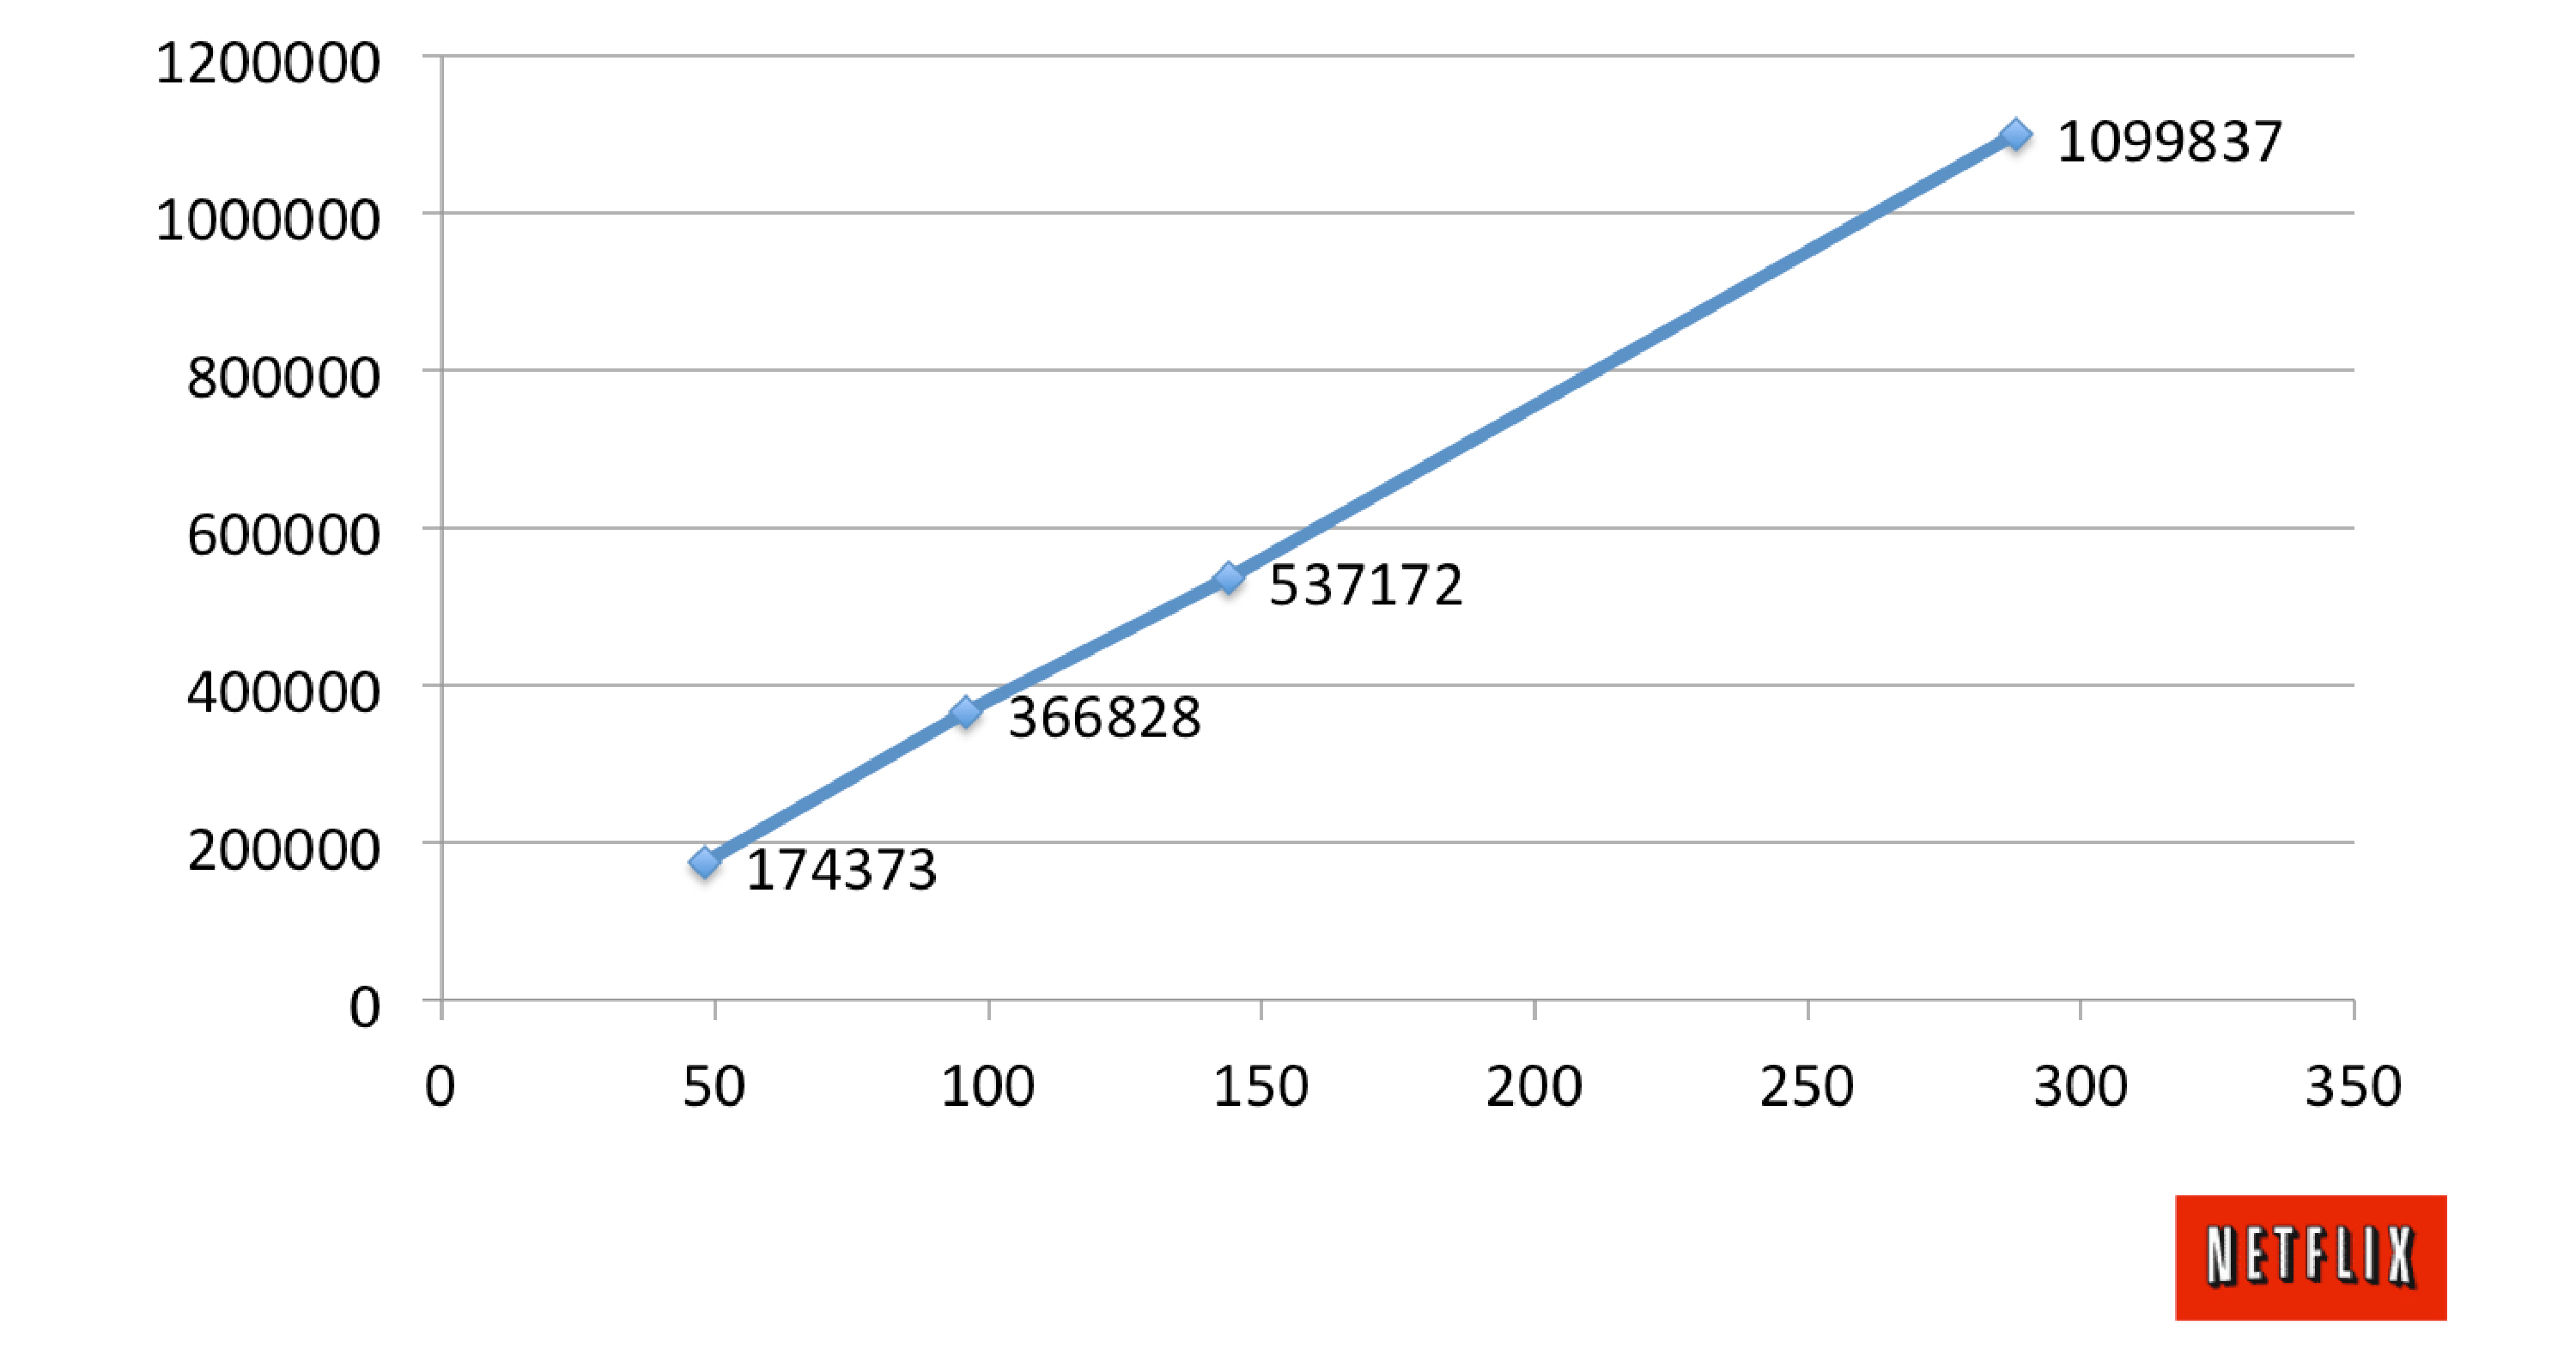
\includegraphics[width=\textwidth]{figure_2.pdf}
  \caption{Netflix experimental data on write throughput of its Cassandra database (Client writes/s by node count; Replication Factor=$3$).
  The x-axis is number of nodes; the y-axis is writes per second.
  From~\cite{cockcroft2011benchmarking}.}
  \label{fig:cassandra_throughput}
\end{figure}


Consider other properties of modern databases:
individual records can be fairly large (megabytes)
and total storage capacity can grow as you add more nodes
(to petabytes and beyond).
Transaction latency can be hundreds of milliseconds
in a globe-spanning distributed database
(and milliseconds in a single data center,
determined mostly by the speed of light).
Moreover, all modern databases have support
for rich querying and permissions.

We never mentioned cost above, but that's also important!
As of early 2017,
if you wanted a short Bitcoin transaction confirmation time,
you had to pay around 25~US~cents
in transaction fees~\cite{bitcoin_tx_fees_2017}.
That works out to around 1~US~cent
per byte of arbitrary data stored,
or ten million US dollars per gigabyte.
Compare that to the cost of Amazon Glacier (used
for long-term, secure, durable data storage):
currently $0.004$~US~dollars per gigabyte-month,
so 40~US~dollars to store a gigabyte for 10000~months
(i.e.~long enough to be effectively forever).
(That's assuming storage costs will stay constant,
but in fact they will go down over time.)

There are many proposals to tweak or improve Bitcoin and similar blockchains,
to increase throughput, increase scalability, increase storage capacity, or reduce latency.
In short, they start with a blockchain and add database characteristics.


\section{The BigchainDB Solution}

BigchainDB takes a different approach.
It's built by starting with a big-data database,
then adding blockchain characteristics
including decentralization, immutability and
built-in support for creation \&~transfer of assets.


\begin{table}[!ht]
  \footnotesize
  \makebox[\textwidth][c]{
  \centering
  \setlength\extrarowheight{3pt}
  \begin{tabular}{ | >{\raggedright}m{\dimexpr 0.25\linewidth-2\tabcolsep} |
	  >{\centering\arraybackslash}m{\dimexpr 0.25\linewidth-2\tabcolsep} |
	  >{\centering\arraybackslash}m{\dimexpr 0.25\linewidth-2\tabcolsep} |
	  >{\centering\arraybackslash}m{\dimexpr 0.25\linewidth-2\tabcolsep} |} \Xhline{4\arrayrulewidth}
  \rowcolor{black} & \color{white} Typical Blockchain & \color{white} Typical Distributed Database & \color{white} BigchainDB \\\Xhline{4\arrayrulewidth}
  High Throughput; increases with node count      &   		           & \checkmark                  & \checkmark          \\\hline
  Low Latency                                     &   		           & \checkmark                  & \checkmark          \\\hline
  High Capacity; increases with node count        &   		           & \checkmark                  & \checkmark          \\\hline
  Rich querying                                   &   		           & \checkmark                  & \checkmark          \\\hline
  Rich permissioning                              &   		           & \checkmark                  & \checkmark          \\\hline
  Decentralization                                & \checkmark 		   &                            & \checkmark          \\\hline
  Immutability                                    & \checkmark 		   &                            & \checkmark          \\\hline
  Built-in support for creation \& transfer of assets & \checkmark     &                            & \checkmark          \\ \Xhline{4\arrayrulewidth}
  \end{tabular}
  }
  \label{tab:bigchain_comparison}
\end{table}


Currently, one can use MongoDB or RethinkDB as the database backend,
but we recommend MongoDB:
a trusted, enterprise-grade database with
high perfomance, strong consistency and modern tooling~\cite{mongodb}.
Figure~\ref{fig:system_diagram} illustrates the architecture
of a BigchainDB cluster.
An external client can communicate with any instance of BigchainDB Server
in the cluster.
Each BigchainDB Server instance is associated with one node
in a MongoDB database.


\begin{figure}[!ht]
  \centering
  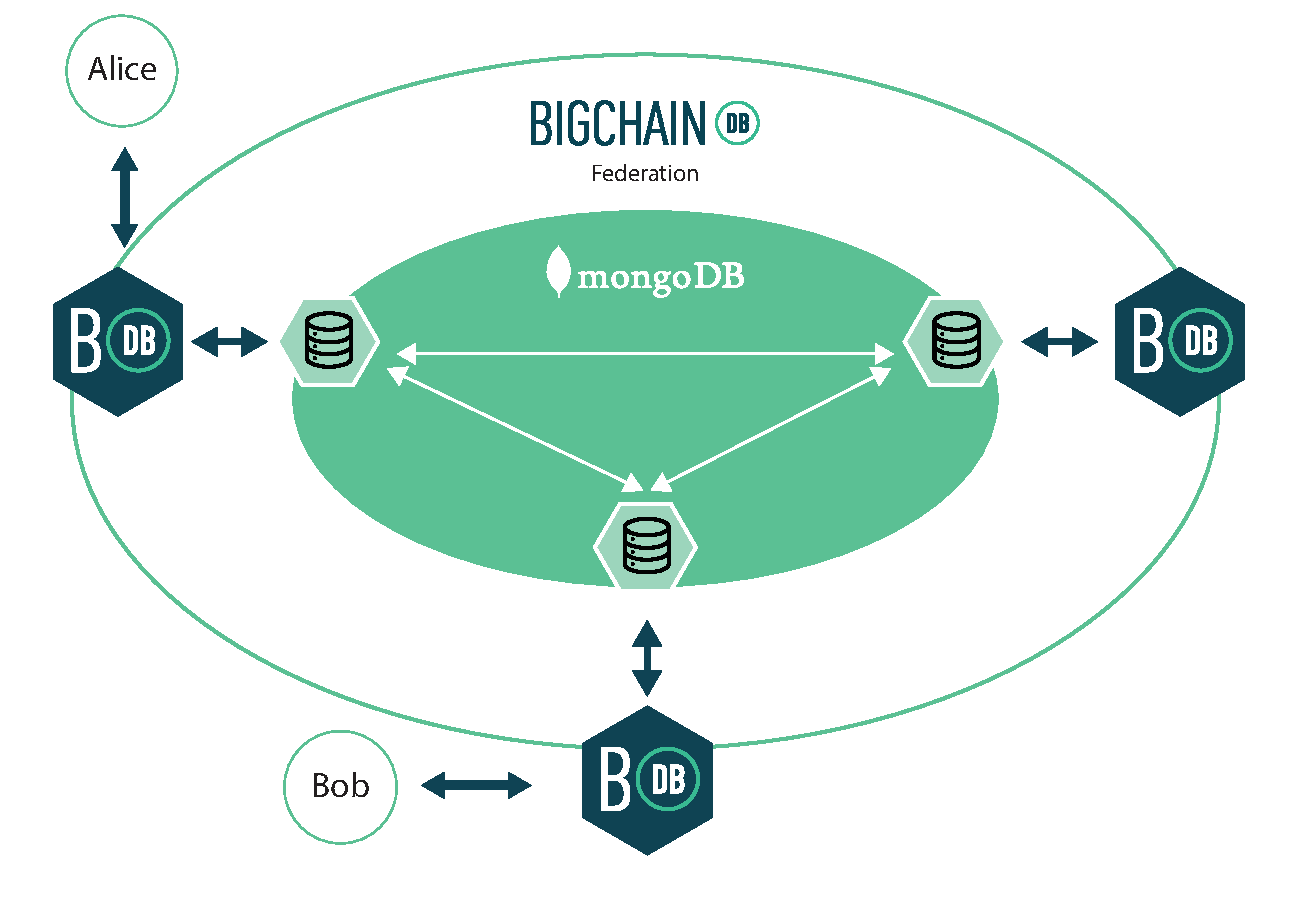
\includegraphics[width=\textwidth]{MDB_BDB_ellipses.pdf}
  \caption{BigchainDB has a client-server architecture.}
  \label{fig:system_diagram}
\end{figure}


\noindent \textbf{Decentralization.}
One key requirement is that every node in the cluster should be owned and operated
by a different person or organization.
That's not handled by the code;
it's something that must be enforced by the organization overseeing
the BigchainDB cluster.
That organization needs rules and processes, for example,
to add and remove participants/nodes (i.e.~governance is required).
The degree of democracy/autocracy can vary from organization to organization.
Ideally, the nodes should be in many countries, legal jurisdictions and hosting providers,
so an issue with one doesn't affect them all.
As with other blockchains,
the only people who can create a valid transfer transaction
are the people with the necessary private keys.
Nobody else, including node operators, can do that:
the power to transact is decentralized.
Plans for adding other decentralizing features
are outlined in the BigchainDB roadmap~\cite{bigchaindb_roadmap}.

\vspace{1 em}

\noindent \textbf{Immutability.}
Blockchains are very tamper-resistant.
Even if tampering does happen, it can be detected
(and rejected),
mostly because of extensive use of cryptographic signatures,
hash chains and Merkle trees.
In the blockchain community,
these characteristics are often called ``immutability''
(which is different from the usual meaning of that word,
but language is a living thing,
and words often get overloaded with additional meanings).
BigchainDB also makes extensive use
of cryptographic signatures and hashes.
For example, all transactions,
blocks and votes are signed.
Also, transactions and blocks are identified
by their hashes.
Tamper-resistance is also increased
by having multiple copies of the data
(i.e.~a high replication factor).
It's worth noting that tamper-resistance can also be augmented
by standard techniques such as secure backups
and secure cluster infrastructure (secure network, secure operating system, etc.).
Plans for adding other tamper-resistance features
are outlined in the BigchainDB roadmap~\cite{bigchaindb_roadmap}.

\vspace{1 em}

\noindent \textbf{Built-in support for creation \& transfer of assets.}
While banks use databases for the transfer of assets all the time,
the databases themselves don't usually have any built-in concept of assets:
that functionality is added in the application layers.
Like most blockchains,
BigchainDB \emph{does} have a built-in concept of assets,
along with built-in
transaction validity checking
(e.g.~checking signatures,
checking for double-spending,
checking that the output-being-spent is in a valid transaction, etc.).

\vspace{1 em}

\noindent \textbf{Sybil tolerance.}
Some blockchain networks (such as Bitcoin) allow anyone
to add their node to the network.
That brings the concern that someone could add
so many nodes that they effectively control the network.
It's known as a Sybil attack.
Bitcoin makes Sybil attacks unlikely by making them
prohibitively expensive.
In a BigchainDB network,
the governing organization behind the network
controls the member list,
so Sybil attacks aren't an issue.


\section{BigchainDB in the Decentralization \mbox{Ecosystem}}

BigchainDB is complementary to decentralized processing / smart contracts (e.g.~Ethereum~\cite{ethereum,buterin-ethereum} or Enigma~\cite{enigma,zyskind2015enigma}), decentralized file systems (e.g.~IPFS~\cite{ipfs}), and communication building blocks (e.g.~email).
It can be included in higher-level decentralized computing platforms (e.g.~Monax/Tendermint~\cite{monax,tendermint}).
It can be used side-by-side with identity protocols, financial asset protocols (e.g.~Bitcoin~\cite{nakamoto2009bitcoin}), intellectual property asset protocols (e.g.~SPOOL~\cite{dejonghe_spool}), and glue protocols (e.g.~pegged sidechains~\cite{back2010sidechains}, Interledger~\cite{thomas2015interledger}).
Scalability improvements to smart contracts blockchains will help fully decentralized applications to better exploit the scalability properties of BigchainDB.

BigchainDB works with more centralized computing systems as well.
One use case is where decentralizing just storage brings the majority of the benefit.
Another use case is where scalability needs are greater than the capabilities of existing decentralized processing technologies; in this case BigchainDB provides a bridge to an eventual fully-decentralized system.

Figure~\ref{fig:bigchain_ecosystem} illustrates how BigchainDB can be used in a fully decentralized setting, or as a mild extension from a traditional centralized computing context.


\begin{figure}[!ht]
  \centering
  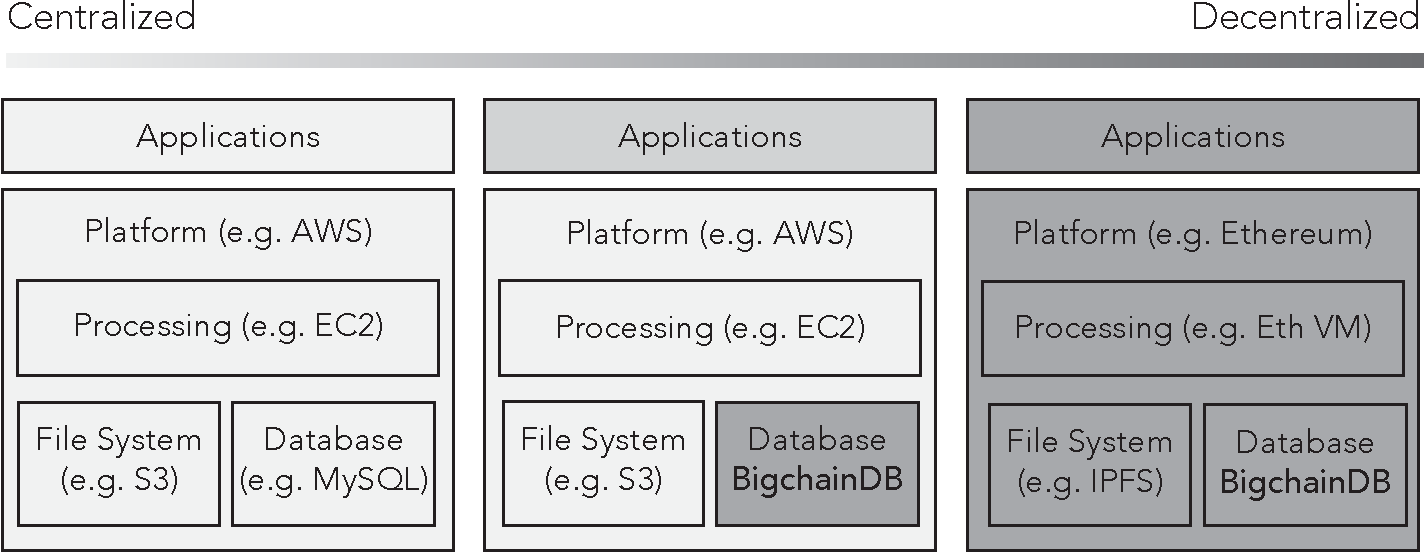
\includegraphics[width=\textwidth]{figure_1.pdf}
  \caption{From a base context of a centralized cloud computing ecosystem (left), BigchainDB can be added as another database to gain some decentralization benefits (middle).
  It also fits into a full-blown decentralization ecosystem (right).}
  \label{fig:bigchain_ecosystem}
\end{figure}


\section{How to Try BigchainDB}

If you want to try BigchainDB,
then you need a BigchainDB cluster to connect to.
One option is to install a single-node BigchainDB ``cluster''
on your local machine.
The Quickstart page
in the BigchainDB Server docs~\cite{bigchaindb_server_quickstart}
has installation instructions.
Another option is to connect to an exsiting
BigchainDB cluster, such as the IPDB Test Network
(IPDB being the Interplanetary Database,
which is managed by the IPDB Foundation\cite{ipdb_foundation_website}).

Once you have a BigchainDB cluster to connect to,
you can communicate with it via the BigchainDB HTTP API~\cite{bigchaindb_http_api}.
BigchainDB also has a WebSocket Event Stream API~\cite{bigchaindb_websocket_api}.
Crafting a valid BigchainDB transaction
(to send to the cluster) is somewhat tricky.
Fortunately, there are many tools and libraries to help:
a CLI, a Python driver, a JavaScript transaction builder, a Java driver, a Go driver, etc.
Links to those are given in the Drivers \& Clients page of the docs~\cite{bigchaindb_drivers_clients}.
Listing~\ref{py1} shows some example example Python code
using the BigchainDB Python driver~\cite{bigchaindb_python_driver}.


\begin{minipage}{\linewidth}
  \begin{lstlisting}[caption={Example Code Using the Python Driver}, label={py1}, style=python]
  from bigchaindb_driver import BigchainDB
  from bigchaindb_driver.crypto import generate_keypair
  bdb = BigchainDB('http://example-bdb-cluster.net:9984')
  alice = generate_keypair()
  golf_club = {
      'data': {
          'name': 'Avocado Greens Golf Club',
          'location': 'Pitts Mills',
          'num_holes': 9
      }
  }
  prepared_creation_tx = bdb.transactions.prepare(
      operation='CREATE',
      signers=alice.public_key,
      asset=golf_club)
  fulfilled_creation_tx = bdb.transactions.fulfill(
      prepared_creation_tx,
      private_keys=alice.private_key)
  sent_creation_tx = bdb.transactions.send(fulfilled_creation_tx)\end{lstlisting}
\end{minipage}

\medskip

Line~4 generates a public/private keypair for a user named \texttt{alice}.
Lines~5--11 create a Python dict named \texttt{golf\_club}.
Lines~12--15 create a raw (unsigned) BigchainDB CREATE transaction,
to create an asset based on the \texttt{golf\_club} dict, for \texttt{alice}.
Lines~16--18 sign that transaction using the private key (signing key)
of \texttt{alice}. Line~19 sends that to the BigchainDB cluster.

There's more example code
in the Python driver docs~\cite{bigchaindb_python_driver}.


\section{Going to Production}

As noted earlier, a production BigchainDB cluster should be operated
by several different people or organizations.
For example, within a single enterprise,
each node could be operated by a different business unit.
Each operator must install and run a ``BigchainDB node''
containing an instance of BigchainDB Server,
an instance of MongoDB (server),
storage for MongoDB,
and potentially other components.
The BigchainDB docs give more details~\cite{bigchaindb_prod_nodes}.


\section{Conclusion}

Many applications could use something decentralized like Bitcoin,
but capable of storing large amounts of arbitrary data quickly,
immutably, and with low latency.
BigchainDB is our answer to that challenge:
a big-data database with blockchain characteristics
including decentralization, immutability and
built-in support for creation \&~transfer of assets.

For more information, see the BigchainDB website
at \href{https://www.bigchaindb.com/}{bigchaindb.com}.


\bibliographystyle{unsrt} %entries will appear in order of their first citation
\bibliography{bigchain}

\end{document}
